% ================================
% INTRODUCTION
% ================================
\section{Introduction}
\label{sec:introduction}

The piezoresistive effect arises from the coupling between mechanical deformation 
and electrical conduction. In typical applications, a doped semiconductor element 
(such as silicon) is embedded within a mechanical structure, where external forces 
induce strain in the material. This deformation alters the electronic transport properties 
of the material, leading to measurable changes in its electrical response, commonly observed 
as variations in voltage or resistance.

\begin{figure}[htbp]
    \centering
    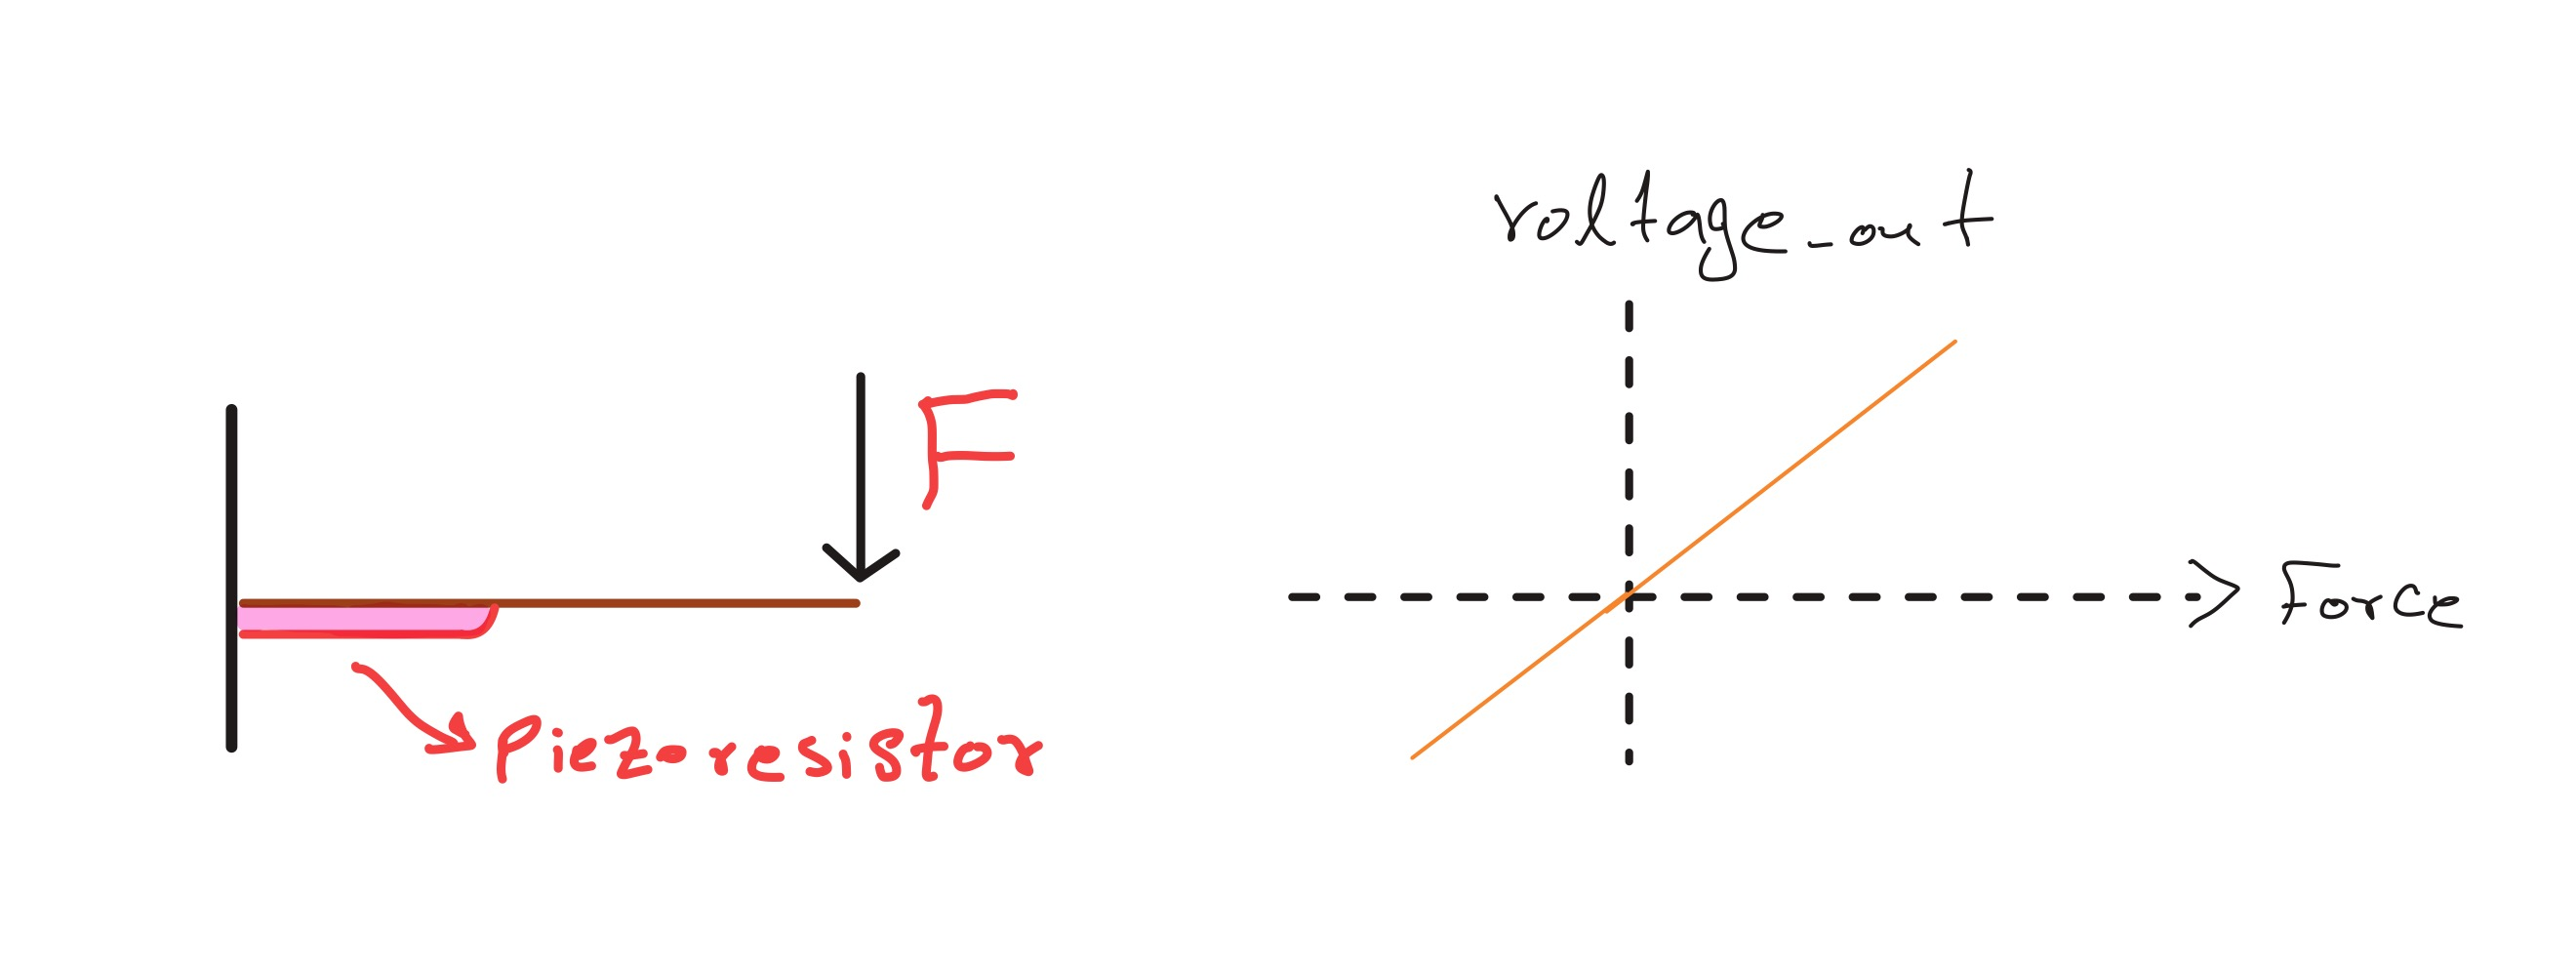
\includegraphics[width=0.5\textwidth]{Images/phenomenon.jpeg}
    \caption{A schematic representation of the piezoresistive effect, where mechanical deformation leads to changes in electrical response.}
\end{figure}

The piezoresistive effect, first observed by William Thomson (Lord Kelvin) 
in the 19th century and later developed for semiconductors by Bardeen, Shockley, and Smith \cite{smith1954}, 
describes the dependence of electrical conductivity on mechanical deformation. 
At a microscopic level, this behavior originates from strain-induced modifications of the electronic structure 
and carrier transport mechanisms. In particular, quantities such as band energies, effective masses, and 
scattering processes are affected by deformation, which in turn influence carrier mobility and conductivity \cite{hamaguchi}.

There exists a wide spectrum of engineering realizations of the piezoresistive effect, 
including strain gauges, pressure sensors, microelectromechanical systems (MEMS), 
cantilever-based sensing devices, and flexible or wearable systems \cite{doll2013}. 
Although these systems differ in geometry, material composition, and boundary conditions, 
they can be interpreted as different realizations of the same underlying electromechanical coupling.

Despite extensive technological development and optimization, the modeling of this coupling 
is often carried out in a phenomenological and application-specific manner, where the dependence 
of conductivity on strain is introduced empirically. From a computational materials perspective, 
this raises a more fundamental question: how can such macroscopic descriptions be related in a 
consistent way to the underlying physical mechanisms governing electronic transport?

The present work approaches this problem by developing a computational framework in which 
the electromechanical coupling is described at the continuum level, while maintaining a clear 
connection to the underlying transport physics. In this setting, the continuum model serves as 
an effective description of strain-dependent conductivity, acting as a bridge between microscopic 
electronic behavior and macroscopic response.

